\section{Metoda niejawna drugiego rzędu}
%%%%%%%%%%%%%%%%%%%%%
\begin{frame}{Metoda}
	$$u^{n+1} = u^n - [f(u^n,t^n)+f(u^{n+1},t^{n+1})]\cdot \frac{\Delta t}{2}$$
    \newline
    - $u^{n+1}$ - uwikłane
    \newline
    - metoda ma dokładność 2-go rzędu
\end{frame}
%%%%%%%%%%%%%%%%%%%%%
\begin{frame}{Stabilność}
	$$g = 1-\frac{\partial f}{\partial u}\bigg\arrowvert_n \cdot\frac{\Delta t}{2}-\frac{\partial f}{\partial u}\bigg\arrowvert_{n+1}\cdot \frac{\Delta t}{2} g$$
	$$g=\frac{1-\frac{\partial f}{\partial u}\arrowvert_n \cdot \frac{\Delta t}{2}}{1+\frac{\partial f}{\partial u}\arrowvert_{n+1} \cdot \frac{\Delta t}{2}}$$
    \begin{figure}
    	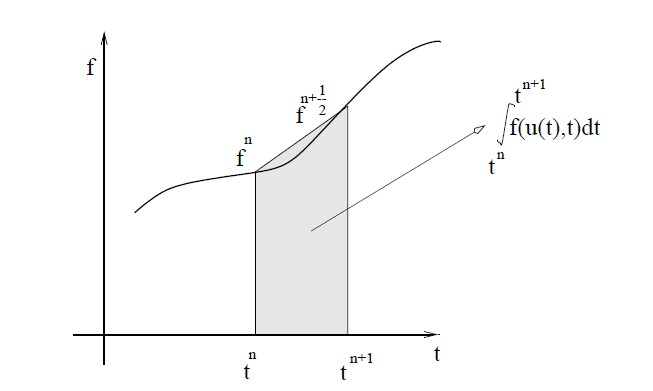
\includegraphics[height=0.55\textheight]{img/22/stabilnosc.jpg}
    \end{figure}
\end{frame}
%%%%%%%%%%%%%%%%%%%%%
\begin{frame}{Stabilność c.d.}
	- równanie rozpadu: $\frac{\partial f}{\partial u} > 0$, \quad $|g| < 1$ (zawsze)
    \newline
    - równanie oscylacyjne $\frac{\partial f}{\partial u}$ - urojone, $|g| = 1$
    \newline\newline
    W obu przypadkach metoda stabilna niezależnie od wyboru kroku
    \begin{itemize}
      \item bezwzględnie stabilna, ważne w zagadnieniach nieliniowych
      \item cena: konieczność rozwiązywania równania algebraicznego na $u^{n+1}$ lub stosowania wzoru iteracyjnego.
    \end{itemize}
\end{frame}
%%%%%%%%%%%%%%%%%%%%%
